\ifdefined\mainfile\else\documentclass{article}% ============================================================
%  FÆLLES PRÆAMBEL
%  Deles af main.tex (hele rapporten) og de enkelte sektionsfiler,
%  som via \ifdefined\mainfile også kan kompileres alene.
%  Ret kun pakker/stil her ét sted.
%  NB: \documentclass er IKKE her -- den står i main.tex (og i sektionernes
%  standalone-guard), så Overleaf ikke forveksler preamble.tex med hoveddokumentet.
% ============================================================
\usepackage[utf8]{inputenc}
\usepackage[T1]{fontenc}
\usepackage[danish]{babel}
\usepackage{subcaption}
\usepackage{graphicx}              % Indsættelse af billeder
\usepackage[absolute,overlay]{textpos}
\usepackage{float}                 % H-placering
\usepackage{amsmath}
\usepackage{amssymb}
\usepackage{siunitx}               % \SI{15}{\volt} m.m. -- praktisk til måleresultater
\usepackage{booktabs}
\usepackage[a4paper, left=2.5cm, right=2.5cm, top=2.5cm, bottom=2.5cm]{geometry}
\usepackage{listings}              % Kildekode-listings
\usepackage{xcolor}
\usepackage{tikz}
\usetikzlibrary{automata, positioning, arrows, calc, shapes.geometric}
\tikzset{
    >=stealth,
    shorten >=2pt, shorten <=2pt,
    node distance=2.8cm,
    block/.style={draw, very thick, rectangle, minimum height=1cm, minimum width=2cm, fill=blue!10},
}
\usepackage[colorlinks=true,
            linkcolor=black,
            citecolor=blue,
            urlcolor=blue]{hyperref}

% ------------------------------------------------------------
%  Listing-stil til C / Arduino-firmware
% ------------------------------------------------------------
\lstdefinestyle{c}{
    language=C,
    basicstyle=\footnotesize\ttfamily,
    keywordstyle=\color{blue}\bfseries,
    commentstyle=\color{green!60!black}\itshape,
    stringstyle=\color{red},
    numbers=left, numberstyle=\tiny\color{gray}, stepnumber=1, numbersep=8pt,
    showspaces=false, showstringspaces=false, showtabs=false,
    frame=single, rulecolor=\color{black}, tabsize=4, captionpos=b,
    breaklines=true, breakatwhitespace=false,
    literate=%
        {æ}{{\ae}}1 {ø}{{\o}}1 {å}{{\aa}}1
        {Æ}{{\AE}}1 {Ø}{{\O}}1 {Å}{{\AA}}1,
}

% ------------------------------------------------------------
%  Listing-stil til MATLAB
% ------------------------------------------------------------
\lstdefinestyle{matlab}{
    language=Matlab,
    basicstyle=\footnotesize\ttfamily,
    keywordstyle=\color{blue}\bfseries,
    commentstyle=\color{green!60!black}\itshape,
    stringstyle=\color{magenta},
    numbers=left, numberstyle=\tiny\color{gray}, numbersep=8pt,
    showstringspaces=false, frame=single, tabsize=4, captionpos=b, breaklines=true,
}

\title{Elektrisk Energisystem}
\author{Gruppe \textbf{XX} -- 62768}
\date{Juni 2026}

% \mainfile defineres i main.tex (IKKE her) -- ellers tror standalone-sektioner
% også at de er i hoveddokumentet og springer deres \end{document} over.
\newcommand{\doubleunderline}[1]{\underline{\underline{#1}}}
\begin{document}\fi

\section{System overview and requirements}
\label{sec:systemoverblik}
% Overordnet blokdiagram (se TikZ-skabelon nedenfor) + de vigtigste krav (V1/V2/V3).
% Forklar energistrømmen: AC-generator -> transformer -> ensretter -> buck;
% solcelle -> MPPT -> lineær reg -> energilager; boost -> pulserende last.

% --- Skabelon til blokdiagram (udfyld/erstat) ---
\begin{figure}[H]
    \centering
    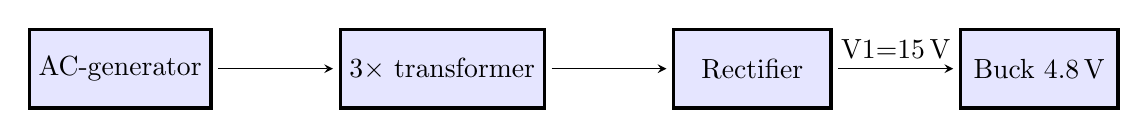
\begin{tikzpicture}[node distance=2.2cm and 1.6cm]
        \node[block] (gen)  {AC-generator};
        \node[block, right=of gen] (tr) {3$\times$ transformer};
        \node[block, right=of tr] (rec) {Rectifier};
        \node[block, right=of rec] (buck) {Buck 4.8\,V};
        \draw[->] (gen) -- (tr);
        \draw[->] (tr) -- (rec);
        \draw[->] (rec) -- node[above]{V1=15\,V} (buck);
    \end{tikzpicture}
    \caption{Simplified block diagram of the energy system, expanded with PV module/MPPT, energy storage, boost converter, and load).}
    \label{fig:blokdiagram}
\end{figure}

\begin{table}[H]
    \centering
    \begin{tabular}{c l l}
        \toprule
        \textbf{Node} & \textbf{Voltage} & \textbf{Requirement} \\
        \midrule
        V1 & 15\,V $\pm$1\,V  & at 100--300\,mA, hold within for 1.0\,s \\
        V2 & 10\,V $\pm$1\,V  & deliver $\geq$150\,mA, last-step 50--150\,mA \\
        V3 & 5\,V $\pm$0.5\,V & for currents $>$20\,mA \\
        \bottomrule
    \end{tabular}
    \caption{Central voltage specifications. Full list in appendiks~\ref{sec:kravsporing}.}
    \label{tab:krav-overblik}
\end{table}

\ifdefined\mainfile\else\end{document}\fi
